\documentclass[12pt, a4paper]{article}
\usepackage[T2A]{fontenc}
\usepackage{amsfonts}
\usepackage{amsmath}
\usepackage{mathabx}
\usepackage{graphicx}
\usepackage{hyperref}
\usepackage{listings}
\usepackage{color}
\usepackage{nicefrac}
\usepackage{tikz}

\title{Теория вероятности 1 модуль.}
\author{Андрей Тищенко БПИ231 @AndrewTGk}
\date{2024/2025}

\begin{document}
    \maketitle
    \begin{center}
        \textbf{Лекция 6 сентября.}
    \end{center}
    \section*{Формула оценки}
    $random()\%11$\\
    $\text{Накоп} = 0.1\text{ИДЗ} + 0.15\text{РС} + 0.25\text{КР} + 0.5\text{Экзамен}$\\
    ИДЗ = индивидуальное домашнее задание (выдаётся через вики курса).
    РС = работа на семинарах.\\
    КР = контрольные работы.
    \begin{center}
        Учебник:
    \end{center}
    Кибзун А. К., Горяинова Е. Р., Наумов А. В. ``Теория 
    вероятности и математическая статистика. Базовый курс 
    с примерами и задачами'' 2013 или 2014 года.
    \section*{История}
    Наука появилась из-за азартных игр. Кавалер Демире захотел составить 
    математическую базу для расчётов в азартных играх. Перечесление многих 
    известных математиков, работавших в этой области. $\underline{\text{Колмогоров}}$ легенда
    теорвера, придумал определение вероятности, основал СУНЦ, ездил на лыжах.\\
    \section*{Основные понятия}
    \subsection*{Определения}
    $\textit{Теория вероятности}$ --- раздел математики, изучающий математические модели массовых случайных явлений.\\
    $\textit{Массовость}$ --- за $n$ повторений эксперимента, вероятность каждого исхода стабилизируется возле какого-то значения $p_i$.\\
    Всякое случайное событие обладает массовостью.
    \subsection*{Обозначения}
    $\omega_1,\dots,\ \omega_n$ --- элементарные случайные события.\\
    $\Omega = \{\omega_1,\dots,\ \omega_n\}$ --- пространство элементарных событий.\\
    $\forall \Omega\ \forall A\quad A\subset \Omega\Leftrightarrow A$ --- случайное событие.\\
    $\forall A\ \forall \Omega\quad  \Omega\subseteq A\Leftrightarrow A$ --- достоверное событие.\\
    $\forall A\ \forall \Omega\quad \Omega\cap A = \emptyset\Leftrightarrow A$ --- невозможное событие.\\
    \section*{Операции с событиями}
    \begin{center}
        $A,\ B\subset \Omega$
    \end{center}
    \subsection*{Произведение}
        Произведением случайных событий $A,\ B$ называется событие $A\cdot B = A\cap B$
    \subsection*{Сумма}
        Сумма $A + B$ есть событие $A\cup B$.
    \subsection*{Разность}
        Разность множеств $A\setminus B$.
    \subsection*{Дополнение}
        $\overline{A} = \Omega\setminus A$.
    \subsection*{Свойства операций}
    \begin{enumerate}
        \item $A + A = A$
        \item $A\cdot A = A$
        \item $A\cdot \Omega = A$
        \item $A + \Omega = \Omega$
        \item $A + B = B + A$
        \item $A\cdot B = B\cdot A$
        \item $A + (B + C) = (A + B) + C$
        \item $\overline{\overline{A}} = A$
        \item $\overline{\overline{\overline{A}}} = \overline{A}$
        \item $\overline{A + B} = \overline{A}\cdot\overline{B}$
    \end{enumerate}

    \subsection*{Определение}
    Класс подмножнеств $\mathcal{A}$ на пространстве событий $\Omega$ называется 
   $\underline{\text{$\sigma$-алгеброй}}$ событий, если:
    \begin{enumerate}
        \item $\Omega\in \mathcal{A}$
        \item $\forall A\subset\Omega\quad A\in \mathcal{A}\Rightarrow \overline{A}\in\mathcal{A}$
        \item $\forall A_i\ A_1,\dots,\ A_n,\dots \in \mathcal{A}\Rightarrow \displaystyle\sum_{i = 1}^{\infty} A_i\in \mathcal{A} \wedge \prod_{i = 1}^{\infty} A_i\in \mathcal{A}$
    \end{enumerate}
    \subsection*{Классическое определение вероятности}
    Исход = элементарное случайное событие.
    \begin{enumerate}
        \item Конечное число исходов эксперимента.
        \item Исходы взаимно исключающие.
        \item Исходы равновозможны.
    \end{enumerate}
    Тогда $P(A) = \frac{|A|}{|\Omega|}$\\
    $|A|$ - мощность множества исходов, принадлежищих $A$.
    \begin{enumerate}
        \item $P(A) \geq 0$
        \item $P(\Omega) = 1$
        \item $A\cdot B = \emptyset\Rightarrow P(A + B) = P(A) + P(B)$
    \end{enumerate}
    \subsection*{Задача}
    В коробке $10$ красных и $20$ чёрных шаров.\\
    Событие $A = \{\text{вытащить красный шар}\}\Rightarrow P(A) = \frac{|A|}{|\Omega|} = \frac{10}{30} = \frac{1}{3}$
    \begin{center}
        Лекция 13 сентября.
    \end{center}
    \section*{Геометрическое определение вероятности}
    $\Omega$ является подмножеством конечной меры в $\mathbb{R}$ или $\mathbb{R}^2$, или ... или $\mathbb{R}^n$.
    $P(A) = \frac{\mu(A)}{\mu(\Omega)}$, $\mu$ - мера (длина, площадь, n-мерный объём).\\
    Свойства:
    \begin{enumerate}
        \item $P(A) \geq 0\quad \forall A\subseteq \Omega$
        \item $P(\Omega) = 1$
        \item $A\cdot B = \emptyset\Rightarrow P(A + B) = P(A) + P(B)$
    \end{enumerate}
    \subsection*{Задача}
    Ромео и Джульетта хотят встретиться между полуночью и часом ночи, но не могут договориться о времени, поэтому они приходят в произвольный момент времени на этом отрезке и ждут 15 минут, после чего уходят. C какой вероятностью они не встретятся?
    $x$ - время прихода Дж.\\
    $y$ - время прихода Ромео.\\
    Тут должен быть балдёжный график, но писать это долго.\\
    $x,\ y\in [0,\ 1]$, в часах.\\
    $|x - y| \leq \frac{1}{4}\\
    P(\overline{A}) = \frac{\frac{3}{4}\cdot \frac{3}{4}}{1} = \frac{9}{16}\Rightarrow P(A) = 1 - \frac{9}{16} = \frac{7}{16}$.\\
    В этом определении мы избавились от конечности множества исходов.
    \section*{Частотное (статистическое) определение вероятности}
    \subsection*{Определение}
    Пусть опыт проведён $N$ раз, а событие $A$ произошло $n_A$ раз. Тогда $\frac{n_A}{N}$ называется частотой события А.\\
    Тогда вероятность $P(A) = \lim\limits_{N\to\infty} \frac{n_A}{N}$
    \section*{Аксиоматическое определение А. Н. Колмогорова (легенды, миллионера, плейбоя и филантропа)}
    \subsection*{Определение}
    Пусть $\mathcal{A} - \sigma$ алгебра событий на пространстве $\Omega$. Назовём вероятностью числовую функцию $P: \mathcal{A}\to \mathbb{R}^1$, удовлетворяющую следующим аксиомам:
    \begin{enumerate}
        \item $\forall A\in \mathcal{A}\quad P(A) \geq 0$
        \item $P(\Omega) = 1$
        \item $\forall A_1,\dots,\ A_n\in \mathcal{A}\quad (\forall i,\ j\in \mathbb{N}\  A_i\cap A_j \neq \emptyset\Rightarrow i = j)\Rightarrow P\left(\displaystyle \sum_{i = 1}^{\infty}A_i\right) =\\
        = \displaystyle\sum_{i = 1}^{\infty}P(A_i)$
    \end{enumerate}
    \subsection*{Определение}
    Число $P(A),\ A\in \mathcal{A}$ называется вероятностью события $A$.
    \subsection*{Определение}
    $(\Omega, \mathcal{A}, P)$ называется вероятностным пространством.
    \subsection*{Свойства P(A)}
    \begin{enumerate}
        \item $P(A) = 1 - P(\overline{A})$.\\
        $\Omega = A + \overline{A}\wedge A\cap \overline{A} = \emptyset$\\
        $P(\Omega) = P(A + \overline{A}) = P(A) + P(\overline{A})\Rightarrow P(A) = 1 - P(\overline{A})$
        \item $P(\emptyset) = 0$\\
        $\overline{\Omega} = \emptyset\Rightarrow P(\Omega) + P(\emptyset) = 1\Rightarrow P(\emptyset) = 1 - 1 = 0$
        \item $A\subseteq \Omega \wedge B\subseteq \Omega \wedge A\subseteq B\Rightarrow P(A) \leq P(B)$\\
        $B = A + (B\setminus A)\Rightarrow P(B) = P\big( A + (B\setminus A) \big) = P(A) + \underset{\geq 0}{\underbrace{P(B\setminus A)}}\Rightarrow\\
        \Rightarrow P(A) \leq P(B)$
        \item $0\leq P(A)\leq 1$\\
        По первой аксиоме $P(A) \geq 0$\\
        Из третьего $A\subseteq \Omega\wedge \Omega\subseteq \Omega\wedge A\subseteq \Omega\Rightarrow P(A) \leq P(\Omega) = 1$
        \item Формула (теорема) сложения вероятностей:
        \[P(A + B) = P(A) + P(B) - P(A\cdot B)\]
        $\begin{cases}
            A = A\cdot \Omega = A\cdot (B + \overline{B}) = AB + A\overline{B}\Rightarrow P(A\overline{B}) = P(A) - P(AB)\\
            B = B\cdot \Omega = B\cdot (A + \overline{A}) = BA + B\overline{A}\Rightarrow P(B\overline{A}) = P(B) - P(AB)
        \end{cases}\Rightarrow\\
        \Rightarrow A + B = AB + A\overline{B} + B\overline{A}\Rightarrow P(A + B) =\\
        = P(AB) + P(A) - P(AB) + P(B) - P(AB) = P(A) + P(B) - P(AB)$\\
        Замечание: тут не было $2(AB)$, потому что сложение по определению есть объединение, поэтому одного экземпляра достаточно.\\
        Для трёх слагаемых:\\
        $P((A + B) + C) = P(A + B) + P(C) - P\big((A + B)\cdot C\big) =\\
        = P(A) + P(B) - P(AB) + P(C) - P(AC) - P(BC) + P(ABC)$\\
        $\displaystyle P(A_1 + \dots + A_n) = \sum_{i = 1}^{n} P(A_i) - \sum_{i \leq j} P(A_i A_j) + \sum_{i\leq j \leq k} P(A_i A_j A_k) +\dots\\
        \dots + (-1)^{n - 1}P(A_1,\dots,\ A_n)$
    \end{enumerate}
    \subsection*{Задача}
    $A_1 = \{\text{Решка при 1-ом броске}\},\ A_2 = \{\text{Решка при 2-ом броске}\}$\\
    $P(A_1 + A_2) = P(A_1) + P(A_2) - P(A_1 A_2) = \frac{1}{2} + \frac{1}{2} - \frac{1}{4} = \frac{3}{4}$
    \subsection*{Определение}
    Пусть $P(B)\neq 0$, тогда условная вероятность события $A$ при условии $B$\\
    \[P(A/B) = \frac{P(AB)}{P(B)}\]
    \subsection*{Определение}
    События $A,\ B$ называются независимыми, если $P(A/B) = P(A)$\\
    Отсюда следует: $\frac{P(AB)}{P(B)} = P(A)\Rightarrow P(AB) = P(A)P(B)$
    \subsection*{Определение}
    События $A_1,\ A_2,\dots,\ A_n$ называются независимыи в совокупности, если:
    \[\forall k = 2,\dots,\ n\ \forall i_1,\dots,\ i_k\quad (1\leq i_1\leq\dots\leq i_k\leq n)\Rightarrow P(A_{i_1},\dots,\ A_{i_k}) = P(A_{i_1})\cdot_{\dots}\cdot P(A_{i_k})\]
    \begin{center}
        Лекция 20 сентября.
    \end{center}
    \subsection*{Воспоминания}
    $P(A/B) = \frac{P(AB)}{P(B)},\quad P(AB) = P(B)P(A/B) = P(A)P(B/A)$
    \section*{Теорема об умножении вероятностей}
    Пусть $(P(A_1,\dots,\ A_n)) > 0$, тогда:
    \[P(A_1,\dots,\ A_n) = P(A_1)P(A_2/A_1)P(A_3/A_1 A_2)\dots P(A_n/A_1\dots A_{n - 1})\]
    \subsection*{Доказательство}
    $\begin{cases}
        B_{n - 1} = A_1\dots A_{n - 1}\\
        B_{n - 2} = A_1\dots A_{n - 2}\\
        \dots\\
        B_{1} = A_1
    \end{cases}\Rightarrow P(\underset{B_{n - 1}}{\underbrace{A_1\dots A_{n - 1}}} A_n) = P(\underset{B_{n - 2} A_{n - 1}}{\underbrace{B_{n - 1}}})P(A_n/ B_{n - 1}) =\\
    = P(B_{n - 2} A_{n - 1})P(A_n/A_1\dots A_{n - 1}) = P(B_{n - 2})P(A_{n - 1}/B_{n - 2})P(A_n/A_1\dots A_{n - 1}) = \\
    = P(A_1)P(A_2/A_1)P(A_3/A_1 A_2)\dots P(A_n/A_1\dots A_{n - 1})$
    \section*{Схема Бернулли (Биномиальная схема)}
    Последовательность испытаний, такая что:
    \begin{enumerate}
        \item Исход любого испытания двоичен $\forall A\ A\vee \overline{A} \equiv 1$
        \item Испытания независимы в совокупности.
        \item $P(A) = p$ не изменяется от опыта к опыту.
    \end{enumerate}
    Например, подбрасывание монеты.\\
    Положим У - успех, Н - неудача.\\
    В таком случае k успехов можно получить $P_n(k)  C_n^k p^k (\underset{ =q}{\underbrace{1 - p}})^{n - k}$ способами
    \subsection*{Доказательство}
    $P(\underset{k}{\underbrace{\text{У}\dots\text{У}}}\underset{n - k}{\underbrace{\text{Н}\dots \text{Н}  }}) = p^k q^{n - k}\\
    P(\{\underset{k}{\underbrace{\text{У}\dots\text{У}}} \text{Н}\dots\text{Н} \}) + P(\text{Н} \underset{k}{\underbrace{\text{У}\dots\text{У}}} \text{Н}\dots \text{Н}) + \dots + P(\text{Н}\dots\text{Н}\underset{k}{\underbrace{\text{У}\dots\text{У}}}) = \\
    = C_n^k p^k q^{n - k}\\
    \displaystyle \sum_{k = 0}^{n} C_n^k p^k q^{n - k} = 1$
    \subsection*{Следствие}
    При $k_1 \leq k \leq k_2:\quad P_n(k) = \displaystyle\sum_{k = k_1}^{k_2}C_n^k p^k q^{n - k}$\\
    \subsection*{Обозначение}
    Если максимальная вероятность достигается при $k = m$, то есть 
    \[C_n^m p^m q^{n - m} = \max\limits_{0\leq k \leq n} C_n^k p^k q^{n - k}\]
    Тогда можно сказать $m = \underset{0 \leq k \leq n}{\operatorname{argmax}} P_n(k)$\\
    Можно посчитать без вычисления всех значений:\\
    $m = \begin{cases}
        [(n + 1) p], \text{ если $(n + 1)p$ - нецелое число}\\
        (n + 1)p \wedge (n + 1)p - 1, \text{ иначе}
    \end{cases}$
    \section*{Полиномиальная схема испытаний}
    \begin{enumerate}
        \item Проводится $n$ независимых опытов
        \item В каждом опыте $m$ взаимноисключающих исходов $(n_1,\dots,\ n_m)$
        \item  $P(n_1) = p_1,\ P(n_2) = p_2,\dots,\ P(n_m) = p_m,\quad p_1 + p_2 + \dots + p_m = 1$
    \end{enumerate}
    $\displaystyle\sum_{i = 1}^{m}  n_i = n\\
    P_n(n_1,\ n_2,\dots,\ n_m) = \frac{n!}{n_1!\, n_2!\dots n_m!}p_1^{n_1}p_2^{n_2}\dots p_m^{n_m}$
    \subsection*{Определение}
    Пусть $H_1,\dots,\ H_n\subset \Omega$, события $H_1,\dots,\ H_n$ называются полной группой событий (гипотезами), если
    \begin{enumerate}
        \item $\forall i,\ j\quad i\neq j\Rightarrow H_i\cdot H_j  = \emptyset$
        \item $H_1 + \cdots + H_n = \Omega$
    \end{enumerate}
    \subsection*{Формула полной вероятности}
    Пусть $H_1,\dots,\ H_n$ --- полный граф событий, $A\subset \Omega$\\
    $P(A) = P(A\cdot \Omega) = P\big(A\cdot (H_1 + \cdots + H_n)\big) = P(AH_1 + \dots + AH_n)$, так как события $H_1,\dots,\ H_n$ независимы, можно сделать переход:\\
    $P(AH_1 + \cdots + AH_n) = P(AH_1) + \cdots + P(AH_n)
    = P(H_1)P(A/H_1) +\\ \dots + P(H_n)P(A/H_n)$\\
    Получаем $P(A) = P(H_1)P(A/H_1) + \cdots + P(H_n)P(A/H_n)$
    \subsection*{Задача}
    Студент выучил $m$ билетов из $n$. Посчитать вероятность вытянуть выученный билет при заходе первым, вторым.\\
    $A = \{\text{студент вытащит выученный билет}\}$\\
    $H_1 = \{\text{Другой студент вытащит выученный нашим студентом билетом}\}\\
    H_2 = \{\text{Наш студен вытащит невыученный билет}\}$\\
    $P(H_1) = \frac{m}{n},\quad P(H_2) = \frac{n - m}{n}\\
    P(A/H_1) = \frac{m - 1}{n - 1},\quad P(A/H_2) = \frac{m}{n - 1}\\
    P(A) = P(H_1)P(A/ H_1) + P(H_2)P(A/H_2) = \frac{m}{n}\frac{m - 1}{n - 1} + \frac{n - m}{n}\frac{m}{n - 1} = \frac{m}{n}$
    \section*{Формула Байeса}
    $H_1,\dots H_n$ --- гипотезы\\
    $P(H_1),\dots,\ P(H_n)$ --- априорные вероятности.\\
    Произошло событие $A$\\
    $P(H_1/A),\dots,\ P(H_n/A)$ --- апосториорные вероятности.\\
    $\displaystyle P(H_i/A) = \frac{P(H_i A)}{P(A)} = \frac{P(H_i)P(A/H_i)}{\sum\limits_{k = 1}^{n} P(H_k) P(A/H_k)}\\
    \sum_{i = 1}^{n} P(H_i/ A) = 1$
    \begin{center}
        Лекция 27 сентября
    \end{center}
    $H_1,\dots,\ H_n$ --- ПГС\\
    $P(H_1),\dots,\ P(H_n)$ --- априорные вероятности.\\
    Произошло событие $A$.\\
    $P(H_1/A),\dots,\ P(H_n/A)$ --- апостериорные вероятности.\\
    $P(H_i/A) = \frac{P(H_i)P(A/H_i)}{\sum_{i = 1}^{n} P(H_n)P(A/H_k)}$\\
    \subsection*{Задача}
    Завод 1 поставляет $65\%$ продукции. При этом $90\%$ его продукции не имеет дефектов.\\
    Завод 2 поставляет $35\%$ продукции. При этом $80\%$ его продукции не имеет дефектов.\\
    Какой завод более вероятно поставит продукт с дефектом?\\
    $A = \{\text{Произведён дефектный продукт}\}\\
    H_1 = \{\text{Прибор изготовил завод 1}\},\ P(H_1) = 0.65,\ P(A/H_1) = 0.1\\
    H_2 = \{\text{Прибор изготовил завод 2}\},\ P(H_2) = 0.35,\ P(A/H_2) = 0.2\\
    P(H_1/A) = \frac{P(H_1) P(A/H_1)}{P(H_1)P(A/H_1) + P(H_2)P(A/H_2)} = \frac{0.1\cdot 0.65}{0.1\cdot 0.65 + 0.2\cdot 0.35} = \frac{65}{135}\\
    P(H_2/A) = \frac{70}{135} > P(H_1/A)$, получается деталь с дефектом с большей вероятностью поступила со второго завода.\\
    \section*{Случайные величины}
    $\Omega = \{\omega_1,\ \omega_2,\dots,\ \omega_6\}\\
    \xi = \{1,\ 2,\dots,\ 6\}\\
    \Omega = \{\omega_1,\ \omega_2,\ \omega_3,\dots\}\\
    \xi = \{1,\ 2,\ 3,\dots\}$\\
    Я понятия не имею, что значат эти множества, но на доске мы их написали со словами: "Давайте покидаем монетку".\\
    Случайная величина $\xi: \Omega\longrightarrow R^1$
    \subsection*{Определение}
    \underline{Случайной величиной} $\xi$ называется числовая функция $\xi: \Omega\longrightarrow R^1$, которая удовлетворяет условию:
    \[\forall x\ \{\omega;\ \xi(\omega) \leq x\} \in \mathcal{A}\]
    \subsection*{Определение}
    \underline{Функцией распределения} (вероятностей) случайной величины $\xi$ называется
    \[F_{\xi}(x) = P(\omega;\ \xi(\omega) \leq x) = P(\xi \leq x)\]
    \begin{center}
        Свойства $F(x)$
    \end{center}
    \begin{enumerate}
        \item $F(+\infty) = 1,\ F(-\infty) = 0\Rightarrow 0\leq F(x) \leq 1$. На самом деле аргумент $F(x)$ принадлежит $R^1$, но видимо бесконечность теперь число.
        \item Пусть $x_1 < x_2$, тогда $F(x_1) \leq F(x_2)$.\\
        Доказательство:\\
        $F(x_2) = P(\xi \leq x_2),\ C = \{\omega:\ \xi(\omega) \leq x_2\},\ A = \{\omega: \xi(\omega) \leq x_1\},\\
        B = \{\omega: x_1 < \xi(\omega) \leq x_2\}.\ C = A + B,\ P(C) = P(A) + P(B)\\
        F(x_2) = P(\xi \leq x_2) = P(\underset{A}{\underbrace{\xi \leq x_1}}) + P(B) = F(x_1) + P(B)\Rightarrow\\
        \Rightarrow F(x_2) \geq F(x_1)$
        \item $F(x_0) = \lim\limits_{\underset{\varepsilon > 0}{\varepsilon \to 0}} F(x_0 + \varepsilon)$
    \end{enumerate}
    \subsection*{Определение}
    \underline{Дискретная случайная величина} (тут реально ничего не было даже на лекции).
    \subsection*{Определение}
    Пусть случайная величина $\xi$ --- дискретная. \underline{Рядом распределения} $\xi$ называется
    \[
    \begin{tabular}{c|c|c|c|c}
      $\xi$ & $x_1$ & $x_2$ & $\dots$ & $x_n$\\
      \hline
      P & $p_1$ & $p_2$ & $\dots$ & $p_n$  
    \end{tabular}\]
    $\displaystyle \sum_{k = 1}^{n} p_k = 1,\ p_k = P(\omega: \xi(\omega) = x_k)$
    \subsection*{Пример}
    $\begin{tabular}{c|c|c|c}
        $\xi$ & -1 & 0 & 2\\
        \hline
        P & 0.3 & 0.5 & 0.2
    \end{tabular}$\\
    Если $x < -1$, то $F(x) = 0$\\
    Если $-1 \leq x < 0$, то $F(x) = 0.3$\\
    Если $0 \leq x < 2$, то $F(x) = 0.8$\\
    Если $2\leq x$, то $F(x) = 1$
    \subsection*{Определение}
    \underline{Математическим ожиданием} (средним значением) дискретной случайной величины с конечным числом значений $x_1,\dots,\ x_n$ называется число
    \[E\xi = \sum_{i = 1}^{n} x_i p_i\]
    Если у дискретной случайной величины счётное количество значений, тогда
    \[E\xi = \sum_{i = 1}^{\infty} x_i p_i,\ \text{если ряд $\displaystyle\sum_{i = 1}^{\infty} |x_i|p_i$ сходится}\]
    Сходимость к $\infty$ считают неопределённой, а с $+\infty,\ -\infty$ проблем нет.
    \subsection*{Определение}
    \underline{Дисперсией} случайной велиины $\xi$ называют
    \[\mathcal{D}\xi = E(\xi - E\xi)^2\]
    Квадрат отклонения от среднего.
    \subsection*{Определение}
    \underline{Среднеквадратическим отклонением} случайной величины $\xi$ называют
    \[\sigma_1 = \sqrt{\mathcal{D}\xi}\]
    \begin{center}
        Свойства математического ожидания
    \end{center}
    \begin{enumerate}
        \item $\forall c\in \mathbb{R}\quad Ec = c$
        \item $E(c\cdot \xi) =\displaystyle \sum_{i = 1}^{n} cx_i p_i = cE\xi$
        \item $\forall a,\ b\in \mathbb{R}\quad a \leq \xi \leq b\Rightarrow a \leq E\xi \leq b$\\
        Доказательство:\\
        $\displaystyle a \leq \sum_{i = 1}^{n} ap_i \leq E\xi = \sum_{i = 1}^{n} x_i p_i \leq \sum_{i = 1}^{n} b p_i = b$
        \item $E(\xi_1 + \xi_2) = E\xi_1 + E\xi_2$
    \end{enumerate}
    \begin{center}
        Лекция 4 октября.
    \end{center}
    Воспоминания:
    \[\begin{tabular}{c|c|c|c}
        $\xi$ & $x_1$ & $\dots$ & $x_n$\\
        \hline
        $p$ & $p_1$ & $\dots$ & $p_n$
     \end{tabular}\]
     $E\xi = \displaystyle \sum\limits_{i = 1}^{n} x_i p_i$
     \begin{center}
        Свойства математического ожидания (продолжение)
     \end{center}
     \begin{enumerate}
        \item[5.] Пусть $\eta = \varphi(\xi),\ \varphi(x)$ - детерминированная функция.\\
        $E\xi = \displaystyle\sum\limits_{i = 1}^{n} \varphi(x_i) p_i$
     \end{enumerate}
     \begin{center}
        Свойства дисперсии.
     \end{center}
     \begin{enumerate}
        \item $\mathcal{D} c = 0$
        \item $\mathcal{D}(c\xi) = E(c\xi - cE\xi)^2 = Ec^2(\xi - E\xi)^2 = c^2\mathcal{D}\xi$
        \item $\forall \xi\quad \text{случайная величина}(\xi)\Rightarrow \mathcal{D}\xi \geq 0$
        \item $\mathcal{D}\xi = E\big(\xi^2 - 2\xi E\xi + (E\xi)^2\big) = E\xi^2 - 2(E\xi)^2 + (E\xi)^2 = E\xi^2 - (E\xi)^2$
        \item $\mathcal{D}(\xi_1 + \xi_2) = E(\xi_1 + \xi_2)^2 - \big(E(\xi_1 + \xi-2)\big)^2 = \\
        = E\xi_1^2 + 2 E(\xi_1\xi_2) + E\xi_2^2 - \big( (E\xi_1)^2 + 2E\xi_1 E\xi_2 + (E\xi_2)^2 \big) = \\
        = \big(E\xi_1^2 - (E\xi_1)^2\big) + \big(E\xi_2^2 - (E\xi_2)^2\big) + 2\big( E(\xi_1 \xi_2) - E\xi_1 E\xi_2 \big) =\\
        = \mathcal{D}\xi_1 + \mathcal{D}\xi_2 + 2\underset{\text{Ковариация } \xi_1 \text{ и } \xi_2}{\underbrace{\big(E(\xi_1 \xi_2) - E\xi_1 E\xi_2\big)}}$\\
    \end{enumerate}
    Если $\xi_1,\ \xi_2$ независимы, то $\operatorname{cov}(\xi_1,\ \xi_2) = 0$ (ковариация нулевая).
    \subsection*{Определение}
    \underline{Начальным моментом k-го порядка} случайной величины $\xi$ называется
    \[\mu_k = E\xi^k,\ k = 1,\ 2,\dots\]
    \subsection*{Определение}
    \underline{Центральным моментом k-го порядка} случайной величины $\xi$ называется
    \[\nu_k = E(\xi - E\xi)^k,\ k = 2,\ 3,\dots\]
    \[\nu_2 = \mathcal{D}\xi\]
    \subsection*{Определение}
    Случайная величина $\overset{\circ}{\xi} = \xi - E\xi$ называется \underline{центрированной} случайной величиной
    \[E\overset{\circ}{\xi} = 0\]
    \subsection*{Определение}
    Случайная величина $\xi^* = \frac{\overset{\circ}{\xi}}{\sigma}$ называют \underline{нормированной} случайной величиной.
    \[D\xi^* = 1\]
    \begin{center}
        Распределения:
    \end{center}
    \begin{enumerate}
        \item Распределение Бернулли
        \[\xi \sim \operatorname{Ber}(p),\quad 0 < p < 1\]
        \[\begin{tabular}{c|c|c}
            $\xi$ & $0$ & $1$\\
            \hline
            $p$ & $1 - p$ & p
        \end{tabular}\quad \begin{tabular}{c|c|c}
            $\xi^2$ & $0$ & $1$\\
            \hline
            $p$ & $1 - p$ & p
        \end{tabular}\]
        \[E\xi = p,\quad \mathcal{D}\xi = E\xi^2 - (E\xi)^2 = p - p^2 = p(1 - p) = pq\]
        \item Биномиальное распределение
        \[\xi \sim \operatorname{Bi}(n,\ p),\quad 0 < p < 1\]
        \[\begin{tabular}{c|c|c|c|c}
            $\xi$ & $0$ & $1$ & $k$ & $n$\\
            \hline
            $p$ & $\dots$ & $\dots$ & $C_n^kp^k q^{n - k}$ & $\dots$
        \end{tabular}\]
        \[E\xi = \sum_{k = 0}^{n}kC_n^k p^k q^{n - k} = \sum_{k = 0}^{n} k\frac{n!}{k!(n - k)!}p^k q^{n - k} =\]
        \[= np\sum_{k = 1}^{n} \frac{(n - 1)!}{( k - 1)!(n - k)!} p^{k - 1}q^{n - k} = \left< \begin{matrix}
            j = k - 1\\
            k = j + 1
        \end{matrix} \right> =\]
        \[=np\sum_{j = 0}^{n - 1} \frac{(n - 1)!}{j!(n - 1 - j)!} p^j q^{n - 1 - j} = np(p + q)^{n - 1} = np\]
        Можно посчитать математическое ожидание иначе:
        \[\xi = \xi_1 + \dots + \xi_n,\quad \begin{tabular}{c|c|c}
            $\xi_i$ & 0 & 1\\
            \hline
            p & $q$ & $p$
        \end{tabular}\Rightarrow E\xi = E\left(\sum\limits_{i = 1}^{n} \xi_i\right) = \sum\limits_{i = 1}^{n} E\xi_i = np\]
        \[\mathcal{D}\xi = \sum_{k = 0}^{n}k^2 C_n^k p^k q^{n - k} - (np)^2 = \dots = npq\]
        Так как $\xi_1,\dots,\ x_n$ независимы:
        \[\mathcal{D}\left( \sum\limits_{i = 1}^{n} \xi_i \right) = \sum_{i = 1}^{n} \mathcal{D}\xi_i = npq\]
        \item Распределение Пуассона
        \[\xi\sim \Pi(\lambda),\quad \lambda > 0\]
        \[\xi = \{0,\ 1,\ 2,\dots\}\]
        \[P(\xi = k) = \frac{e^{-\lambda} \lambda^k}{k!}\]
        \[\sum_{k = 0}^{\infty} = \sum_{k = 0}^{\infty}\frac{e^{-\lambda}\lambda^k}{k!} = e^{-\lambda}\sum_{k = 0}^{\infty}\frac{\lambda^k}{k!} = e^{-\lambda} e^{\lambda} = 1\]
        \[E\xi = \sum_{k = 0}^{\infty} k \frac{e^{-\lambda}\lambda^k}{k!} = e^{-\lambda}\lambda\sum_{k = 1}^{\infty}\frac{\lambda^{k - 1}}{(k - 1)!} = \lambda e^{-\lambda}e^{\lambda} = \lambda\]
        \[\mathcal{D}\xi = E\xi^2 - (E\xi)^2 = \sum_{k = 0}^{\infty} k^2\frac{e^{-\lambda}\lambda^k}{k!} - \lambda^2 = \lambda \sum_{k = 1}^{\infty} k \frac{e^{-\lambda}\lambda^{k - 1}}{(k - 1)!} - \lambda^2=\]
        \[=\lambda\sum_{k = 1}^{\infty} (k - 1 + 1) \frac{e^{-\lambda} \lambda^{k - 1}}{(k - 1)!} - \lambda^2 = \lambda^2 + \lambda - \lambda^2 = \lambda\]
    \end{enumerate}
    \subsection*{Теорема Пуассона}
    Пусть в схеме испытаний Бернулли: $n\to \infty,\ p\to 0,\ np\to \lambda$. Тогда 
    \[\lim_{n\to\infty}C_n^k p^k q^{n - k} = \frac{e^{-\lambda}\lambda^k}{k!}\]
    \subsection*{Доказательство}
    \[\lim_{n\to\infty}C_n^k p^k q^{n - k} = \lim_{n\to \infty} \frac{n!}{k!(n - k)!}\left( \frac{\lambda}{n} \right)^k\left( 1 - \frac{\lambda}{n} \right)^{n - k}=\]
    \[= \frac{\lambda^k}{k!} \lim_{n\to \infty} \frac{n(n - 1)\dots(n - k + 1)}{n^k} \frac{(1 - \frac{\lambda}{n})^n}{(1 - \frac{\lambda}{n})^k} = \frac{\lambda^k}{k!}e^{-\lambda}\]
    Погрешность такой апроксимации:
    \[\left|C_n^k p^k q^{n - k} - \frac{e^{-np}(np)^k}{k!}\right| \leq np^2\]
    \subsection*{Задача}
    Завод поставляет 1000 бутылок воды. Каждая бутлка может быть повреждена в пути с вероятностью $0.002$. Какое среднее количество бутылок будет повреждено? Какова вероятность повреждения не более 2 бутылок?\\
    Случайная величина $\xi$ --- количество повреждённых бутылок.\\
    $\xi \sim \operatorname{Bi}(1000, 0.002)\Rightarrow E\xi = 1000\cdot 0.002 = 2$\\
    Погрешность при апроксимации Пуассоновским распределением будет $\leq np^2 = 0.004$, что нас устраивает по точности.\\
    $P(\xi \leq 2) = p(\xi = 0) + p(\xi = 1) + p(\xi = 2) = e^{-2}(1 + 2 + 2) = \frac{5}{e^2}$
    \begin{center}
        Ещё распределения
    \end{center}
    \begin{enumerate}
        \item[4.] Геометрическое распределение
        \[\xi\sim G(p),\quad 0 < p < 1\]
        $\xi = \{1,\ 2,\dots\},\quad P(\xi = k) = q^{k - 1}p$. После первого успеха эксперименты прекращаюся.\\
        \[E\xi = \sum_{k = 1}^{\infty} k q^{k - 1} p = p \sum_{k = 1}^{\infty} k q^{k - 1} = p \sum_{k = 1}^{\infty}\left( q^k \right)' = p\left( \sum_{k = 1}^{\infty} q^k \right)' =  p\left( \frac{q}{1 - q} \right)' =\]
        $\dfrac{p}{p^2} = \dfrac{1}{p}$
    \end{enumerate}
    \subsection*{Задача}
    Студент выучил 80\% билетов. Преподаватель спрашивает его, пока не обнаружит незнание. Сколько в среднем билетов спросит преподаватель?\\
    $\xi \sim G(0.2)\quad E\xi = \frac{1}{0.2} = 5$

    \begin{center}
        Лекция 11 октября.
    \end{center}
    Воспоминания: $F_{\xi}(x) = P(\xi \leq x)$
    \begin{center}
        \section*{Непрерывные случайные величины}
    \end{center}
    \subsection*{Определение}
    Неотрицательная кусочно-непрерывная функция $f_{\xi}(x)$ называется \underline{плотностью} \underline{распределения} случайной величины $\xi$, если
    \[F_{\xi}(x) = \int\limits_{-\infty}^{x} f_{\xi}(t)\, dt\]
    Прикол про Канторову лестницу:\\
    $F(x) = \begin{cases}
        0,\ x\leq 0\\
        \frac{1}{2}F(3x),\ 0\leq x < \frac{1}{3}\\
        \frac{1}{2},\ \frac{1}{2} \leq x < \frac{2}{3}\\
        \frac{1}{2} + \frac{1}{2}F(3x - 2),\ \frac{2}{3} \leq x < 1\\
        1,\ x\geq 1
    \end{cases}$ непрерывна, но не имеет плотности.\\
    $P(\xi = x) = F(x) - \underset{\underset{\varepsilon > 0}{\varepsilon \to 0}}{\lim} F(x - \varepsilon) = 0\\
    f(x) = F'(x) = \lim\limits_{\Delta x \to 0} \frac{F(x + \Delta x) - F(x)}{\Delta x} = \lim\limits_{\Delta x\to 0} \frac{P(x < \xi \leq x + \Delta x)}{\Delta x}\\
    f(x)\Delta x \underset{\Delta x \to 0}{=} P(x < \xi \leq x + \Delta x)$

    \begin{center}
        Свойства $f_{\xi}(x)$
    \end{center}
    \begin{enumerate}
        \item $\forall x\in \mathbb{R}^1\quad f_{\xi}(x) \geq 0$
        \item $\displaystyle \int_{-\infty}^{+\infty} f_{\xi}(x)\, dx = F(+\infty) = 1$
        \item $\displaystyle \int_{x_1}^{x_2} f(x)\, dx = F(x_2) - F(x_1) = P(x_1 < \xi \leq x_2)$
        \item В точках дифференцируемости функции $F(x)$
        \[f(x) = F'(x)\]
        \item Пусть случайная величина $\xi$ имеет плотность распределения $f_{\xi}(x)$. Детерминированная функция $\varphi(x)$ является монотонной и дифференцируемой.
        \[\text{СВ } \eta = \varphi(\xi)\quad f_{\eta}(y) - ?\]
        \begin{enumerate}
            \item[a.] Пусть $\varphi(x)$ --- монотонно возрастающая функция:
            \[F_{\eta}(y) = P(\eta \leq y) = P(\varphi(\xi) \leq y) = P\big(\xi \leq \varphi^{-1}(y)\big) = F_{\xi}\big(\varphi^{-1}(y)\big)\]
            \[f_{\eta}(y) = \frac{d}{dy} F_{\eta}(y) = f_{\xi}\big(\varphi^{-1}(y) \big)\cdot (\varphi^{-1}(y))'\]
            \item[b.] Пусть $\varphi(x)$ --- монотонно убывающая функция.
            \[F_{\eta}(y) = P(\eta \leq y) = P\big(\varphi(\xi) \leq y\big) = P\big(\xi \geq \varphi^{-1}(y)\big) = 1 - F_{\xi}\big(\varphi^{-1}(y)\big)\]
            \[f_{\eta}(y) = \frac{d}{dy} F_{\eta}(y) = - f_{\xi}\big( \varphi^{-1}(y) \big) \big( \varphi^{-1}(y) \big)'\]
            Минус возникает для компенсации отрицательности производной обратной функции.
            \item[c.] Пусть $\varphi(x)$ --- монотонная функция:
            \[f_{\eta}(y) = f_{\xi}\big(\varphi^{-1}(y)\big) \Big| \big( \varphi^{-1}(x) \big)' \Big|\]
            \item[d.] Если $\varphi(x)$ --- немонотонная функция. Разбиваем на интервалы монотонности:
            \[\varphi_1(x),\ \varphi_2(x),\dots,\ \varphi_n(x)\]
            Найдём: $\varphi_1^{-1}(y),\ \varphi_2^{-1}(y),\dots,\ \varphi_n^{-1}(y)$. Тогда:
            \[f_{\eta}(y) = \sum_{i = 1}^{k} f\big( \varphi_i^{-1}(y) \big) \Big|\big( \varphi_i^{-1}(y) \big)'\Big|\]
        \end{enumerate}
    \end{enumerate}

    \subsection*{Определение}
    Математическое ожидание непрерывной случайной величины $\xi$ с плотностью $f_{\xi}(x)$ называется число:
    \[E\xi = \int\limits_{-\infty}^{+\infty} xf_{\xi}(x)\, dx\]
    если сходится $\displaystyle \int\limits_{-\infty}^{+\infty} |x| f_{\xi}(x)\, dx$
    \subsection*{Замечание}
    \begin{enumerate}
        \item Если $f_{\xi}(x) > 0$ только при $x > 0$ и $\displaystyle\int_{-\infty}^{+\infty} x f_{\xi}(x)\, dx$ расходится, то $E\xi = +\infty$
        \item Если $f_{\xi}(x) > 0$ только при $x < 0$ и $\displaystyle\int_{-\infty}^{+\infty} x f_{\xi}(x)\, dx$ расходится, то $E\xi = -\infty$
        \item Распределение Коши: $f(x) = \frac{1}{\pi(1 + x^2)}$
        \[\int\limits_{-\infty}^{+\infty} x \frac{1}{\pi(1 + x^2)} dx\]
    \end{enumerate}\newpage
    \begin{center}
        Совйства математического ожидания
    \end{center}
    \begin{enumerate}
        \item $Ec = c$
        \item $E(c\xi) = cE(\xi)$
        \item $a\leq \xi \leq b\Rightarrow a\leq E\xi \leq b$
        \item $E(\xi_1 + \xi_2) = E\xi_1 + E\xi_2$
        \item Пусть случайная величина $\eta = \varphi(\xi),\ \varphi$ --- детерминированная функция.
        \[E\eta = \int\limits_{\infty}^{\infty} \varphi(x) f_{\xi}(x)\, dx\]
    \end{enumerate}
    \subsection*{Определение}
    Дисперсией называется:
    \[\mathcal{D}\xi = E(\xi - E\xi)^2 = E\xi^2 - (E\xi)^2\]
    \begin{center}
        Квант$\acute{\text{и}}$ль.
    \end{center}
    \subsection*{Определение}   
    Число $\underline{Z_{\gamma}}$ $0 < \gamma < 1$, называется \underline{$\gamma$-квантилью} непрерывного строго монотонного распределения $F_{\xi}(x)$, если:
    \[F_{\xi}(Z_{\gamma}) = \gamma = P(\xi \leq Z_{\gamma}) = \int\limits_{-\infty}^{Z_{\gamma}} f(x)\, dx\]
    Были примеры с графиками, я их очень люблю.
    \subsection*{Определение}
    
    Квантиль $Z_{0,5}$ называется \underline{медианой}. Не всегда совпадает с математическим ожиданием.
    
    \begin{center}
        Лекция 25 октября
    \end{center}
    \subsection*{Равномерное распределение}
    \[\xi\sim R(a,\ b)\]
    $f(x) = \begin{cases}
        0,\ x\notin (a,\ b)\\
        \frac{1}{b - a}, x\in(a,\ b)
    \end{cases}\\
    E\xi = \frac{a + b}{2}\\
    \mathcal{D}\xi = \frac{(b - a)^2}{12}\\
    F(x) = \displaystyle \int\limits_{-\infty}^{x} f(t)\, dt\Rightarrow F(x) = \begin{cases}
        0,\ x\leq a\\
        \frac{x - a}{b - a},\ x\in (a,\ b)\\
        1,\ x\geq b
    \end{cases}$
    \subsection*{Экспоненциальное (показательное) распределение}
    \[\xi \sim E(\lambda),\ \lambda > 0\]
    $f(x) = \begin{cases}
        0,\ x < 0\\
        \lambda e^{-\lambda x},\ x\geq 0
    \end{cases}\\
    E\xi = \frac{1}{\lambda}\\
    \mathcal{D}\xi = \frac{1}{\lambda^2}\\
    F(x) = \begin{cases}
        0,\ x < 0\\
        1 - e^{-\lambda x},\ x\geq 0
    \end{cases}$
    \subsection*{Свойства}
    Пусть $\xi \sim E(\lambda)$, тогда:
    \[\forall t,\ \tau\quad P(\xi > t + \tau / \xi > t) = P(\xi > \tau),\ \text{условная вероятность}\]
    \subsection*{Доказательство}
    $\displaystyle P(\xi > t + \tau / \xi > t) = \frac{P(\xi > t + \tau)}{P(\xi > t)} = \frac{1 - F(t + \tau)}{1 - F(t)} = \frac{e^{-\lambda(t + \tau)}}{e^{-\lambda t}} = e^{-\lambda \tau} =\\
    = 1 - F(\tau) = P(\xi > \tau)$
    \subsection*{Нормальное (гауссовское) распределение}
    \[\xi \sim N(m,\ \sigma^2)\]
    $f(x) = \displaystyle\frac{1}{\sqrt{2\pi}\sigma} e^{-\frac{(x - m)^2}{2\sigma^2}}\\
    E\xi = m\\
    \mathcal{D}\xi = \sigma^2$
    \subsection*{Определение}
    Функция $\Phi_0(x) = \displaystyle \int\limits_{0}^{x} \frac{1}{\sqrt{2\pi}}e^{-\frac{t^2}{2}}\, dt$ называется \underline{функцией Лапласа}
    \subsection*{Свойства}
    $\Phi_0 (+\infty) = 0.5\\
    \Phi_0(-x) = -\Phi_0(x)$\\
    Правило трёх сигм
    \[P(|\xi - m| < 3\sigma) = 2\Phi_0\left( \frac{3\sigma}{\sigma} \right) = 2\Phi_0(3) = 0.997\]
    \begin{center}
        Лекция 1 ноября
    \end{center}
    \subsection*{Неравенства Чебникова}
    Пусть $E|\xi|^r < \infty$. Тогда:
    \[\forall \varepsilon > 0\quad P(|\xi| \geq \varepsilon) \leq \frac{E|\xi|^r}{\varepsilon^r}\]
    \subsection*{Доказательство}
    $E|\xi|^r = \displaystyle\int\limits_{-\infty}^{+\infty} |x|^r f(x)\, dx$
    \\
    \begin{center}
        $x\in (-\infty,\ -\varepsilon] \cup [\varepsilon,\ +\infty)$, то есть\\ 
    \end{center}
        \[\begin{tikzpicture}[transform canvas={scale=1.2}]
            \draw (-1.5, 0) -- node[anchor=north]{$x$} (0, 0);
            \draw (0, 0) -- node[anchor=north]{$x$} (1.5, 0);
            \draw[red] (-0.5, 0) -- (0.5, 0);
            \filldraw (-0.5, 0) circle  (0.25mm) node[anchor=south]{$-\varepsilon$};
            \filldraw (0.5, 0) circle  (0.25mm) node[anchor=south]{$\varepsilon$};
        \end{tikzpicture}\]
    Тогда:\\
    $\displaystyle\int\limits_{-\infty}^{+\infty} |x|^r f(x)\, dx\geq \int\limits_{|x|\geq \varepsilon}^{+\infty} |x|^r f(x)\, dx \geq \varepsilon^r \int\limits_{|x|>\varepsilon}^{+\infty} f(x)\, dx = \varepsilon^r P(|\xi| \geq \varepsilon)\Rightarrow \\
    \Rightarrow\frac{E|\xi|^r}{\varepsilon^r} \geq P(|\xi|\geq \varepsilon)$, ч.т.д.
    \begin{center}
        \underline{Частные случаи}
    \end{center}
    \begin{enumerate}
        \item $r = 1 \wedge P(\xi \geq 0) = 1$
        \[P(\xi \geq \varepsilon) \leq \frac{E\xi}{\varepsilon}\]
        \item Пусть $r = 2$
        \[P(|\xi| \geq \varepsilon) \leq \frac{E\xi^2}{\varepsilon^2}\]
        \item Пусть $r = 2,\quad \eta = \xi - E\xi$
        \[P(|\xi = E\xi| \geq \varepsilon) \leq \frac{\mathcal{D}\xi}{\varepsilon^2}\]
        \subsection*{Задача}
        Случайная величина $\xi$ --- расход электрической энергии в месяц. Известно $E\xi = 4\,000$. Оценить $P(\xi \geq 10\, 000)$.\\
        Применяя неравенство Чебышёва может прикинуть эту вероятность:
        \[P(\xi \geq 10\, 000) \leq \frac{4\, 000}{10\, 000} = 0.4\]
        \textbf{Неравенство не находит вероятность точно, используется только для получения грубой оценки!}
    \end{enumerate}
    \subsection*{Определение}
    Вектор $\xi = (\xi_1,\dots,\ \xi_n)$, компоненты которого $\xi_1,\dots,\ \xi_n$, являющиеся случайными величинами, называется \underline{случайным вектором}.
    \subsection*{Определение}
    Функцией распределения случайного вектора $\xi = (\xi_1,\dots,\ \xi_n)$ называется
    \[F_{\xi}(x_1,\dots,\ x_n) = P(\xi_1 \leq x_1,\dots,\ \xi_n \leq x_n)\]
    \subsection*{Замечание}
    $\{\xi_1 \leq x_1,\dots,\ \xi_n \leq x_n\} = \{(\xi_1\leq x_1)\cap(\xi_2 \leq x_2) \cap \dots \cap (\xi_n \leq x_n)\}$
    \subsection*{Пример}
    Пуcть $n = 2$. $F_{\xi}(x,\ y) = P(\xi_1 \leq x,\ \xi_2 \leq y)$\\
    \begin{center}
        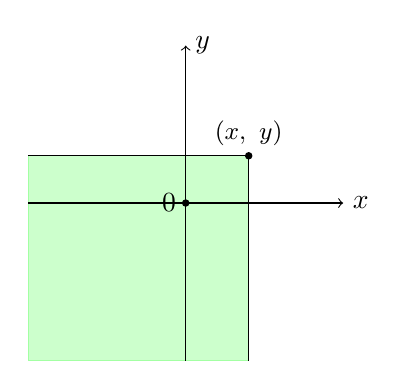
\begin{tikzpicture}[scale=2]
            \filldraw[green, opacity=0.2] (-1, -1) rectangle (0.4, 0.3);
            \draw[->] (0, -1) -- (0, 1) node[anchor=west]{$y$};
            \draw[->] (-1, 0) -- (1, 0) node[anchor=west]{$x$};
            \draw (-1, 0.3) -- (0.4, 0.3);
            \draw (0.4, -1) -- (0.4, 0.3);
            \filldraw (0.4, 0.3) circle(0.2mm) node[anchor=south]{\small$(x,\ y)$};
            \filldraw (0, 0) circle(0.2mm) node[anchor=east]{0};
        \end{tikzpicture}
    \end{center}
    \begin{center}
        \underline{Свойства $F(x,\ y)$}
    \end{center}
    \begin{enumerate}
        \item $\forall x,\ y\quad 0 \leq F(x,\ y) \leq 1$
        \item $F(-\infty,\ -\infty) = 0 = F(x,\ -\infty) = F(-\infty,\ y)$
        \item $F(+\infty,\ +\infty) = 1$
        \item $F(+\infty,\ y) = P(\xi_2 \leq y) = F_{\xi_2}(y)$
    Рассмотрим вероятность попадания в квадрат:\\
    \begin{tikzpicture}[scale=2]
        \draw[->] (0, -1) -- (0, 1) node[anchor=west]{$y$};
        \draw[->] (-1, 0) -- (1, 0) node[anchor=west]{$x$};
        \filldraw (0.4, 0.3) circle(0.2mm) node[anchor=east]{\small$(a_1,\ b_1)$};
        \filldraw (0, 0) circle(0.2mm) node[anchor=east]{$0$};
        \draw (0.4, 0.3) rectangle ++(0.4, 0.2);
        \filldraw (0.8, 0.5) circle(0.2mm) node[anchor=west]{\small$(a_2,\ b_2)$};
        \draw[dashed] (-1, 0.5) -- (0.4, 0.5);
        \draw[dashed] (-1, 0.3) -- (0.4, 0.3);
        \draw[dashed] (0.4, 0.3) -- (0.4, -1);
        \draw[dashed] (0.8, 0.3) -- (0.8, -1);
    \end{tikzpicture}
        \item $P(a_1 \leq \xi \leq a_2,\ b_1 \leq \xi_2 \leq b_2) =\\
        = F(a_2,\ b_2) - F(a_2,\ b_1) - F(a_1,\ b_2) + F(a_1,\ b_1)$
        \item $F(x,\ y)$ монотонно неубывающая функция по каждому аргументу.\\
        \textit{Доказательство:} $\forall \Delta x > 0 \quad F(x + \Delta x,\ y) \geq F(x,\ y)\\
        F_{\xi}(x + \Delta x,\ y) = P(\xi \leq x + \Delta x,\ \xi_2\leq y) = P(\xi_1 \leq x,\ \xi_2 \leq y) +\\
         + \underset{\alpha \geq 0}{\underbrace{P(x < \xi_1\leq x + \Delta x,\ \xi_2 \leq y)}} = F(x,\ y) + \alpha \geq F(x,\ y)$
    \end{enumerate}
    \subsection*{Определение}
    Компоненты $\xi_1$ и $\xi_2$ случайного вектора $\xi = (\xi_1,\ \xi_2)$ называются \underline{независимыми}, если верно:
    \[\forall x,\ y\quad F_{\xi}(x,\ y) = F_{\xi_1}(x)F_{\xi_2}(y)\]
    \subsection*{Определение}
    Дискретный случайный вектор:
    \[\begin{tabular}{|c|c|}
    \hline
    $\xi_1,\ \xi_2$ & $y_1\dots y_k$\\
    \hline
    $x_1$ & $p_{1\, 1}\dots p_{1\, k}$\\ 
    $x_2$ & $p_{2\, 1}\dots p_{2\, k}$\\
    $\vdots$ & $\vdots$\\ 
    $x_n$ & $p_{n\, 1}\dots p_{n\, k}$\\ 
    \hline
    \end{tabular}\]
    $p_{i\, j} = P(\xi_1 = x_i,\ \xi_2 = y_j)\\
    \displaystyle \sum_{i = 1}^{m} \sum_{j = 1}^{k} p_{i\, j} = 1\\
    \begin{tabular}{c|c|c|c|c}
        $\xi_1$ & $x_1$ & $x_2$ & $\dots$ & $x_m$\\
        \hline
        p & $p_{1\textbf{$\bullet$}}$ & $p_{2\textbf{$\bullet$}}$ & $\dots$ & $p_{m\textbf{$\bullet$}}$ 
    \end{tabular}\\
    p_{i\textbf{$\bullet$}} = \sum_{j = 1}^{k} p_{i\, j}$
    \subsection*{Утверждение}
    Компоненты $\xi_1,\ \xi_2$ дискретного случайного вектора $\xi = (x_1,\ x_2)$ независимы тогда и только тогда, когда
    \[\forall i=\overline{1,\ m},\ j=\overline{1,\ k}\quad p_{i\, j} = p_{i\textbf{$\bullet$}}\cdot p_{\textbf{$\bullet$}j}\]
    \subsection*{Определение}
    Неотрицательная кусочно-непрерывная функция $f_{\xi}(x,\ y)$ называется плотностью распределения случайного вектора $\xi = (\xi_1,\ \xi_2)$, если
    \[F_{\xi}(x,\ y) = \int\limits_{-\infty}^{x}\int\limits_{-\infty}^{y} f(t_1,\ t_2)\, dt_2\, dt_1\]
    \subsection*{Замечание}
    В точках дифференцируемости $F(x,\ y)$
    \[f(x,\ y) = \frac{\delta^2 F(x,\ y)}{\delta x\, \delta y},\ \text{$\delta$ частная производная}\]
    \begin{center}
        \underline{Свойства $f(x,\ y)$}
    \end{center}
    \begin{enumerate}
        \item $\forall x,\ y\quad f(x,\ y) \geq 0$
        \item $\displaystyle \int\limits_{-\infty}^{+\infty}\int\limits_{-\infty}^{+\infty} f(x,\ y)\, dx\, dy = F(+\infty, +\infty) = 1$
        \item $\displaystyle \int\limits_{a_1}^{a_2} \int\limits_{b_1}^{b_2} f(x,\ y)\, dy\, dx = F(a_2\, b_2) - F(a_2,\ b_1) - \big(F(a_1,\ b_2) - F(a_1,\ b_1)\big) =\\
        = P(a_1 < \xi_1 \leq a_2,\ b_1 < \xi_2 \leq b_2)$
        \item На доске нарисована клякса $D$, разбитая на много маленьких прямоугольников\\
        $f(\tilde{x},\ \tilde{y}),\ \Delta x,\ \Delta y,\quad \tilde{x} \in (x,\ x + \Delta x),\ \tilde{y} \in (y,\ y + \Delta y)$. Тогда
        \[P(\xi \in D) = \iint_{D} f(x,\ y)\, dx\, dy,\ \text{вспоминаем матан.}\]
        \item $\displaystyle F_{\xi_1}(x) = F_{\xi}(x,\ +\infty) = \int\limits_{-\infty}^{x}\int\limits_{-\infty}^{+\infty} f(t,\ y)\, dy\, dt\\
        f_{\xi_1}(x) = \frac{d}{dx} F_{\xi_1}(x) = \frac{d}{dx} \int\limits_{-\infty}^{x}\int\limits_{-\infty}^{+\infty} f(t,\ y)\, dy\, dt = \int\limits_{-\infty}^{+\infty} f(x,\ y)\, dy\\
        f_{\xi_2}(y) = \int\limits_{-\infty}^{+\infty} f(x,\ y)\, dx$
    \end{enumerate}
    \begin{center}
        Лекция 8 ноября
    \end{center}
    \subsection*{Определение}
    Случайный вектор $\xi = (\xi_1,\dots,\ \xi_n)$ имеет \underline{равномерное распределение} \underline{в области} $\mathcal{D}\in \mathbb{R}^n$, если 
    \[f_{\xi}(x_1,\dots,\ x_n) = \begin{cases}
        c,\ \text{если } (x_1,\dots,\ x_n)\in \mathcal{D}\\
        0,\ \text{иначе}
    \end{cases}, \text{где $c$ --- константа}\]
    \subsection*{Частный случай}
    При $n = 2$ случайный вектор $\xi = (\xi_1,\dots,\ \xi_n)$ распределён равномерно в области $\mathcal{D}$, если 
    \[f_{\xi}(x,\ y) = \begin{cases}
        \frac{1}{S},\ \text{если } (x,\ y)\in \mathcal{D}\\
        0,\ \text{иначе}
    \end{cases},\ \text{где $S$ --- площадь $\mathcal{D}$}\]
    \subsection*{Пример 1}
    Пусть $\xi = (\xi_1,\ \xi_2)$ распределён равномерно в области
    \[f_{\xi}(x,\ y) = \begin{cases}
        1,\ \text{если } x\in (0,\ 1)\wedge y\in(0,\ 1)\\
        0,\ \text{иначе}
    \end{cases}\]
    \[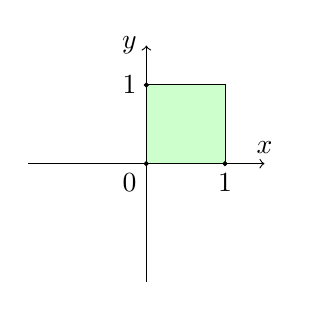
\begin{tikzpicture}
        \draw[->] (0, -1.5) -- (0, 1.5) node[anchor=east]{$y$};
        \draw[->] (-1.5, 0) -- (1.5, 0) node[anchor=south]{$x$};
        \filldraw[green, opacity=0.2] (0, 0) rectangle (1, 1);
        \draw (0, 0) rectangle (1, 1);
        \filldraw (1, 0) circle (0.25mm) node[anchor=north]{1};
        \filldraw (0, 1) circle (0.25mm) node[anchor=east]{1};
        \filldraw (0, 0) circle (0.25mm) node[anchor=north east]{0};
    \end{tikzpicture}\]
    \[f_{\xi_1}(x) = \int\limits_{-\infty}^{+\infty} f_{\xi}(x,\ y)\, dy = \begin{cases}
        \displaystyle\int\limits_0^1 1\, dy,\ \text{если } x\in (0,\ 1)\\
        0,\ \text{если } x\notin(0,\ 1)
    \end{cases} = \begin{cases}
        1,\ \text{если } x\in (0,\ 1)\\
        0,\ \text{если } x\notin(0,\ 1)
    \end{cases} \]
    \[f_{\xi_2}(y) = \int\limits_{-\infty}^{+\infty} f_{\xi}(x,\ y)\, dx = \begin{cases}
        \displaystyle\int\limits_0^1 1\, dx,\ \text{если } y\in (0,\ 1)\\
        0,\ \text{если } y\notin(0,\ 1)
    \end{cases} = \begin{cases}
        1,\ \text{если } y\in (0,\ 1)\\
        0,\ \text{если } y\notin(0,\ 1)
    \end{cases} \]
    Получаем $\forall x,\ y\in \mathbb{R}^2\quad f_{\xi}(x,\ y) = f_{\xi_1}(x)\cdot f_{\xi_2}(y)\Rightarrow$ случайные величины зависимы.
    \subsection*{Пример 2}
    Пусть $\xi = (\xi_1,\ \xi_2)$ распределён равномерно в круге радиуса $R$
    \[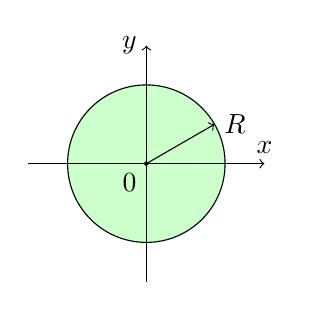
\begin{tikzpicture}
        \filldraw[green, opacity=0.2] (0, 0) circle (1cm);
        \filldraw (0, 0) circle (0.25mm) node[anchor=north east]{0};
        \draw[->] (0, -1.5) -- (0, 1.5) node[anchor=east]{$y$};
        \draw[->] (-1.5, 0) -- (1.5, 0) node[anchor=south]{$x$};
        \draw (0, 0) circle (1cm);
        \draw[->] (0, 0) -- (0.866, 0.5) node[anchor=west]{$R$};
    \end{tikzpicture}\]
    \[f_{\xi}(x,\ y) = \begin{cases}
        \frac{1}{\pi R^2},\ \text{если } x^2 + y^2 \leq R\\
        0,\ \text{иначе}
    \end{cases}\]
    \[f_{\xi_1}(x) = \int\limits_{-\infty}^{+\infty} f(x,\ y)\, dy = \int\limits_{-\sqrt{R^2 - x^2}}^{+\sqrt{R^2 - x^2}} \frac{1}{\pi R^2}\, dy = \begin{cases}
        \frac{2\sqrt{R^2 - x^2}}{\pi R^2},\ \text{если } |x| \leq R\\
        0,\ \text{иначе}
    \end{cases}\]
    \[f_{\xi_1}(y) = \int\limits_{-\infty}^{+\infty} f(x,\ y)\, dx = \int\limits_{-\sqrt{R^2 - y^2}}^{+\sqrt{R^2 - y^2}} \frac{1}{\pi R^2}\, dx = \begin{cases}
        \frac{2\sqrt{R^2 - y^2}}{\pi R^2},\ \text{если } |y| \leq R\\
        0,\ \text{иначе}
    \end{cases}\]
    Получаем $\exists x,\ y\quad f_{\xi}(x,\ y) \neq f_{\xi_1}(x)\cdot f_{\xi_2}(y)\Rightarrow$ случайные величины зависимы.
    \subsection*{Утверждение}
    Пусть $\xi = (\xi_1,\ \xi_2)$ --- непрерывный случайный вектор, тогда $\xi_1$ и $\xi_2$ --- независимы тогда и только тогда, когда
    \[\forall x,\ y\in \mathbb{R}\quad f_{\xi}(x,\ y) = f_{\xi_1}(x) f_{\xi_2}(y)\]
    \subsection*{Доказательство}
    \textbf{``$\Rightarrow$''}\\
    Пусть $\xi_1$ и $\xi_2$ независимы, тогда:
    \[f_{\xi}(x,\ y) = \frac{\delta^2 F(x,\ y)}{\delta x \cdot \delta y} = \frac{\delta^2 F_{\xi_1}(x) F_{\xi_2} (y)}{\delta x \delta y} = \frac{dF_{\xi_1}(x)}{dx}\cdot \frac{dF_{\xi_2}(y)}{dy} = f_{\xi_1}(x)\cdot f_{\xi_2}(y)\]
    \textbf{``$\Leftarrow$''}\\
    Пусть $f_{\xi} (x,\ y) = f_{\xi_1}(x)\cdot f_{\xi_2}(y)$, тогда:
    \[F_{\xi}(x,\ y) = \int\limits_{-\infty}^{x}\int\limits_{-\infty}^{y}f_{\xi}(t,\ s)\, ds\, dt = \int\limits_{-\infty}^{x}\int\limits_{-\infty}^{y} f_{\xi_1}(t)f_{\xi_2}(s)\, ds\, dt = \int\limits_{-\infty}^{x} f_{\xi_1}(t) \left(\int\limits_{-\infty}^{y}f_{\xi_2}(s)\, ds\right)\, dt =\]
    \[= F_{\xi_1}(x) F_{\xi_2}(y)\Rightarrow \xi_1,\ \xi_2\ \text{независимы.}\]
    \subsection*{Определение}
    \underline{Математическим ожиданием вектора} $\xi = (\xi_1,\dots,\ \xi_n)$ называют вектор $E\xi = (m_1,\dots,\ m_n)$, где $\forall i\in \{1,\ 2,\dots n\}\ m_i = E\xi_i$
    \begin{center}
        \textbf{Свойства математического ожидания}
    \end{center}
    \begin{enumerate}
        \item $E(\xi_1 + \xi_2) = E\xi_1 + E\xi_2$\\
        \textit{Доказательство:} $E(\xi_1 + \xi_2) = \displaystyle\sum_i \sum_j (x_i + y_j)p_{i\, j} =\\
        = \sum_{i}\sum_{j} x_i p_{i\, j} + \sum_{i}\sum_{j} y_j p_{i\, j} = \sum_{i} x_i p_{i\, \bullet} + \sum_{j} y_j p_{\bullet\, j} = E\xi_1 + E\xi_2$
        \item $\xi_1,\ \xi_2\ \text{независимы} \Rightarrow E(\xi_1\xi_2) = E\xi_1\cdot E\xi_2$\\
        \textit{Доказательство:} $E(\xi_1\xi_2) = \displaystyle\int\int x y f(x,\ y)\, dx\, dy =\left< \begin{aligned}
            &\text{компоненты $\xi_1,\ \xi_2$}\\
            &\text{независимы}
        \end{aligned} \right> =\\
        = \int\int x y f_{\xi_1}(x) f_{\xi_2}(y)\, dx\, dy = \int\limits_{-\infty}^{+\infty} y f_{\xi_2}(y) \left(\int\limits_{-\infty}^{+\infty} x f_{\xi_1}(x)\, dx\right)\, dy =\\
        = \int\limits_{-\infty}^{+\infty} x f_{\xi_1}(x)\, dx \int\limits_{-\infty}^{+\infty} y f_{\xi_2}(y)\, dy = E\xi_1\cdot E\xi_2$
    \end{enumerate}\
    \subsection*{Определение}
    \underline{Ковариацией} случайных величин $\xi_1,\ \xi_2$ называют величину
    \[\operatorname{cov}(\xi_1,\ \xi_2) = k_{\xi_1\, \xi_2} = E(\xi_1 - E\xi_1)(\xi_2 - E\xi_2) = E\overset{\circ}{\xi_1}\overset{\circ}{\xi_2}\]
    \textit{Напоминание:} $\overset{\circ}{\xi}$ обозначает центрированную случайную величину.
    \subsection*{Определение}
    \underline{Коэффициентом корреляции} случайных величин $\xi_1,\ \xi_2$ называется
    \[\rho_{\xi_1\, \xi_2} = \frac{\operatorname{cov}(\xi_1,\ \xi_2)}{\sqrt{\mathcal{D}\xi_1 \mathcal{D}\xi_2}} = \operatorname{cov}(\xi_1^*,\ \xi_2^*)\]
    \textit{Напоминание:} $\xi^* = \frac{\xi - E\xi}{\sqrt{\mathcal{D}\xi}}$
    \subsection*{Определение}
    Случайные величины $\xi_1,\ \xi_2$ называются\\
    \underline{некоррелированными}, если
    \[\rho_{\xi_1,\ \xi_2} = 0\]
    \underline{Положительно коррелированными}, если
    \[\rho_{\xi_1,\ \xi_2} > 0\]
    \underline{Отрицительно коррелированными}, если
    \[\rho_{\xi_1,\ \xi_2} < 0\]
    \begin{center}
        Свойства $\operatorname{cov}(\xi_1,\ \xi_2)$
    \end{center}
    \begin{enumerate}
        \item $\operatorname{cov}(\xi,\ \xi) = \mathcal{D}\xi$
        \item $\mathcal{D}(\xi + \eta) = \mathcal{D}\xi + \mathcal{D}\eta + 2\operatorname{cov}(\xi,\ \eta)$
        \item $\operatorname{cov}(\xi,\ \eta) = \operatorname{cov}(\eta,\ \xi)$
        \item $\operatorname{cov}(\xi,\ \eta) = E(\xi - E\xi)(\eta - E\eta) = E(\xi\eta) - E\xi\cdot E\eta$
        \item $\operatorname{cov}(a\xi + b,\ c\eta + d) = E(a\xi + b - aE\xi - b)(c\eta + d - cE\eta - d) = a\cdot c \operatorname{cov}(\xi,\ \eta)$
        \item $|\rho_{\xi\, \eta}| = \frac{|\operatorname{cov}(\xi,\ \eta)|}{\sigma_{\xi}\sigma_{\eta}} \leq 1\Rightarrow |\operatorname{cov}(\xi,\ \eta)| \leq \sigma_{\xi}\sigma_{\eta}$\\
        \textit{Доказательство:}\\
        $0\leq \mathcal{D(\xi^* + \eta^*)} = \mathcal{D}\xi* + \mathcal{D}\eta^* + 2\overset{=\rho_{\xi^*\, \eta^*}}{\overbrace{\operatorname{cov}(\xi^*,\ \eta^*)}} = 1 + 1 + 2\rho_{\xi^*\, \eta^*} =\\
        = 2(1 + \rho_{\xi^*\, \eta^*}) \geq 0\Rightarrow \rho_{\xi^*\, \eta^*} \geq -1$\\
        $0\leq \mathcal{D(\xi^* - \eta^*)} = \mathcal{D}\xi* + \mathcal{D}\eta^* - 2\underset{=\rho_{\xi^*\, \eta^*}}{\underbrace{\operatorname{cov}(\xi^*,\ \eta^*)}} = 1 + 1 - 2\rho_{\xi^*\, \eta^*} =\\
        = 2(1 - \rho_{\xi^*\, \eta^*}) \geq 0\Rightarrow \rho_{\xi^*\, \eta^*} \leq 1$\\
        \item $\xi,\ \eta$ --- независимые случайные величины и $\mathcal{D}\xi,\ \mathcal{D}\eta \in \mathbb{R}$ $\Rightarrow\\
        \Rightarrow \operatorname{cov}(\xi,\ \eta) = 0$\\
        \textit{Доказательство:}
        \[\operatorname{cov}(\xi,\ \eta) = E\overset{\circ}{\xi}\overset{\circ}{\eta} = \int\limits_{-\infty}^{+\infty}\int\limits_{-\infty}^{+\infty} (x - m_{\xi})(y - m_{\eta}) f(x,\ y)\, dx\, dy = \left< \begin{aligned}
            & \text{компоненты $\xi,\ \eta$}\\
            & \text{независимы}
        \end{aligned} \right> =\]
        \[=\int\limits_{-\infty}^{+\infty}\int\limits_{-\infty}^{+\infty} (x - m_{\xi})f(x) (y - m_{\eta})f(y)\, dx\, dy = \int\limits_{-\infty}^{+\infty} (x - m_{\xi})f(x)\, dx \int\limits_{-\infty}^{+\infty} (y - m_{\eta}) f(y)\, dy = 0\]
        0 получается, потому что\\
        $\displaystyle\int\limits_{-\infty}^{+\infty} (x - m_{\xi})f(x)\, dx = \underset{=E\xi}{\underbrace{\int\limits_{-\infty}^{+\infty}xf(x)\, dx}} - m_{\xi}\underset{=1}{\underbrace{\int\limits_{-\infty}^{+\infty}f(x)\, dx}} = E\xi - E\xi = 0$
    \end{enumerate}
    \begin{center}
        Лекция 15 ноября
    \end{center}
    \begin{center}
        \textbf{Свойства $\rho_{\xi,\, \eta}$}
    \end{center}
    \begin{enumerate}
        \item $|\rho_{\xi\, \eta}| \leq 1$
        \item $\rho_{\xi\, \xi} = 1$
        \item Если случайная величина $\eta = a\xi + b,\ a\neq 0$, то
        \[\rho_{\xi\, \eta} = \begin{cases}
            1,\ \text{если}\ a > 0\\
            -1,\ \text{если}\ a < 0
        \end{cases}\]
        \textit{Доказательство:}
        \[\rho_{\xi\, \eta} = \frac{\operatorname{cov}(\xi,\ \eta)}{\sqrt{\mathcal{D}\xi\cdot \mathcal{D}\eta}} = \frac{E\xi\eta - E\xi E\eta}{\sqrt{\mathcal{D}\xi\cdot \mathcal{D}\eta}} = \frac{E\xi(a\xi + b) - E\xi E(a\xi + b)}{\sqrt{\mathcal{D}\xi\cdot \mathcal{D}(a\xi + b)}} =\]
        \[=\frac{aE\xi^2 + bE\xi - a(E\xi)^2 - bE\xi}{\sqrt{a^2(\mathcal{D}\xi)^2}} = \frac{a(E\xi^2 - (E\xi)^2)}{|a|\mathcal{D}\xi} = \frac{a\mathcal{D}\xi}{|a|\mathcal{D}\xi} = \begin{cases}
            1,\ \text{если}\ a > 0\\
            -1,\ \text{если}\ a < 0
        \end{cases}\]
        \item Пусть $|\rho_{\xi\, \eta}| = 1\Rightarrow \eta = a\xi + b$
        \begin{enumerate}
            \item[a)] $\rho_{\xi\, \eta} = 1 = \rho_{\xi^*\, \eta^*}$\\
            \[\mathcal{D}(\xi^* - \eta^*) = \mathcal{D}\xi^* + \mathcal{D}\eta^* + 2\operatorname{cov}(\xi^*,\ -\eta^*) = \mathcal{D}\xi^* + \mathcal{D}\eta^* - 2\operatorname{cov}(\xi^*,\ \eta^*) =\]
            \[= 2 - 2\rho_{\xi\, \eta} = 2(1 - \rho_{\xi\, \eta}) = 0\]
            Итак, получаем:
            \[\mathcal{D}(\xi^* - \eta^*) = 0 \Rightarrow \xi^* - \eta^* = c\Rightarrow \frac{\xi - m_{\xi}}{\sigma_{\xi}} - \frac{\eta - m_{\eta}}{\sigma_{\eta}} = c\Rightarrow \text{ линейно зависимы}\]
            \item[б)] $\rho_{\xi\, \eta} = -1$:
            \[\mathcal{D}(\xi^* + \eta^*) = \mathcal{D}\xi^* + \mathcal{D}\eta^* + 2\operatorname{cov}(\xi^*\, \eta^*) = 2(1 + \rho_{\xi\, \eta}) = 0\]
        \end{enumerate}
    \end{enumerate}
    \subsection*{Пример}
    Пусть $\xi \sim R(-a, a)$, $\eta = \xi^2$. Посчитаем коэффициент корелляции:
    \[\operatorname{cov}(\xi,\ \eta) = E\xi \eta - \underset{=0}{\underbrace{E\xi}} E\eta = E\xi^3 = \int\limits_{-a}^{a} x^3 \frac{1}{2a}\, dx = 0\Rightarrow \rho_{\xi\, \eta} = 0\]
    Итого, величины зависимы, но не коррелированы (так как корелляция показывает линейную зависимость, а $\eta$ зависит от $\xi$ квадратично).
    \subsection*{Определение}
    \underline{Ковариационной матрицей} вектора $\xi = \{\xi_1,\dots,\ \xi_n\}$ называется матрица $K_{\xi} = \begin{pmatrix}
        k_{i\, j}
    \end{pmatrix}$, где $k_{i\, j} = \operatorname{cov}(\xi_i,\ \xi_j),\ i,\ j = \overline{1,\ n}$
    \begin{center}
        Свойства $K_{\xi}$
    \end{center}
    \begin{enumerate}
        \item $k_{i\, j} = k_{j\, i}\Rightarrow K_{\xi}$ симметричная
        \item $k_{i\, i} = \mathcal{D}\xi_{i},\ i = \overline{1,\ n}$
        \item $K_{\xi}$ неотрицательно определённая, то есть 
        \[\forall \lambda_1,\dots,\ \lambda_n\in\mathbb{R}\quad \sum_i\sum_j \lambda_i\lambda_j k_{i\, j} \geq 0\]
        \textit{Доказательство:}
        \[0 \leq E\left(\sum_{i = 1}^{n} \lambda_ii \overset{\circ}{\xi_i}\right)^2 = E\left( \sum_i \sum_j \lambda_i \lambda_j \overset{\circ}{\xi_i}\overset{\circ}{\xi_j} \right) = \sum_i \sum_j \lambda_i \lambda_j \underset{k_{i\, j}}{\underbrace{E\overset{\circ}{\xi_i}\overset{\circ}{\xi_j}}}\]
    \end{enumerate}
    \subsection*{Определение}
    \underline{Корреляционной матрицей} случайного вектора $\xi = (\xi_1,\dots,\ \xi_n)$ называется матрица $R_{\xi} = \begin{pmatrix}
        \rho_{i\, j}
    \end{pmatrix}$, где $\rho_{i\, j} = \rho_{\xi_1\, \xi_2}$
    \begin{enumerate}
        \item $\forall i,\ j = \overline{1,\ n}\quad \rho_{i\, j} = \rho_{j\, i}$
        \item $\forall i = \overline{1,\ n}\quad \rho_{i\, i} = 1$
    \end{enumerate}
    \subsection*{Формула свёртки}
    Пусть случайные величины $\xi_1$ и $\xi_2$ --- независимы, $\xi_1\sim f_{\xi_1}(x),\ \xi_2 \sim f_{\xi_2}(y)$\\
    Случайная величина $\eta = \xi_1 + \xi_2$.\\
    Найти: $f_{\eta}(z) - ?$
    \[F_{\eta}(z) = P(\eta \leq z) = P(\xi_1 + \xi_2 \leq z) = \iint\limits_{x + y \leq z} f_{\xi_1}(x) f_{\xi_2}(y)\, dy\, dx = \int\limits_{-\infty}^{+\infty}\int\limits_{-\infty}^{z - x} f_{\xi_1}(x) f_{\xi_2}(y)\, dy\, dx\]
    \[f_{\eta}(z) = \frac{d}{dz} F_{\eta}(z) = \int_{-\infty}^{+\infty} f_{\xi_1}(x)f_{\xi_2}(z - x)\, dx\]
    \subsection*{Пример}
    $\xi_1 \sim N(0,\ 1),\ \xi_2 \sim N(0,\ 1)$\\
    $\xi_1$ и $\xi_2$ --- независимы.\\
    $\eta = \xi_1 + \xi_2,\ f_{\eta}(z) - ?$
    \[f_{\eta}(z) = \int_{-\infty}^{+\infty} \frac{1}{\sqrt{2\pi}} e^{-\frac{x^2}{2}}\cdot \frac{1}{\sqrt{2\pi}} e^{-\frac{(z - x)^2}{2}}\, dx = \int\frac{1}{2\pi}e^{-\frac{x^2}{2} - \left( \frac{z^2}{2} - xz + \frac{x^2}{2} \right)}=\]
    \[=\frac{e^{-\frac{z^2}{4}}}{\sqrt{2\pi}\sqrt{2}} \int\limits_{-\infty}^{+\infty} \frac{1}{\sqrt{2\pi}\sqrt{\frac{1}{2}}} e^{-x^2 + xz - \frac{z^2}{4}} = \frac{e^{-\frac{z^2}{4}}}{\sqrt{2\pi}\sqrt{2}} \underset{=1}{\underbrace{\int\limits_{-\infty}^{+\infty} \frac{1}{\sqrt{2\pi}\sqrt{\frac{1}{2}}} e^{-(x - \frac{z}{2})^2}}}\]
    Равно 1, потому что это гауссовская плотность, тогда оставшаяся часть и будет плотностью распеределения.\\
    Итак, $\eta \sim N(0, 2)$.
    \subsection*{Утверждение}
    Пусть $\xi_1,\dots,\ \xi_n$ --- независимые случайные величины, такие что $\xi_i\sim N(m_i,\ \sigma_i^2),\ i = \overline{1,\ n}$\\
    Тогда случайная величина $\eta = \xi_1 + \dots + \xi_n \sim N(m_{\eta},\ \mathcal{D}\eta)$,\\
    где $\displaystyle m_{\eta} = \sum_{i = 1}^{n} m_i,\ \mathcal{D}\eta = \sum_{i = 1}^{n} \sigma_i^2$
\end{document}